\documentclass[12pt]{article}
\usepackage{geometry}                
\geometry{letterpaper}

\usepackage{graphicx}
\usepackage{amsmath}
\usepackage{amssymb}
\usepackage{amsthm}
\usepackage{amsrefs}
\usepackage{dsfont}
\usepackage{mathrsfs}
\usepackage{stmaryrd}
%\usepackage[all]{xy}
\usepackage[mathcal]{eucal}
\usepackage{verbatim}  %%includes comment environment
\usepackage{fullpage}  %%smaller margins
\usepackage{enumerate}
\usepackage{xltxtra}
\usepackage{fontspec}
\usepackage{xunicode}

\usepackage{listings}
\usepackage{booktabs}
\usepackage{float}
\usepackage{hyperref}
\hypersetup{
    colorlinks,
    citecolor=blue,
    filecolor=blue,
    linkcolor=blue,
    urlcolor=blue
}
\renewcommand{\nobreakspace}{\nobreak\ }


\defaultfontfeatures{Mapping=tex-text}

\usepackage{/usr/local/Cellar/r/2.14.0/R.framework/Resources/share/texmf/tex/latex/Sweave}
\begin{document}
\lstset{language=C,breaklines=true,frame=single,basicstyle=\footnotesize}

\title{cudatrace --- A parallel ray tracer written in CUDA/C}
\author{Dominick LoBraico and Laura Macaddino}
\date{\today}
\maketitle

\begin{abstract}
    \textsc{cudatrace} is a high performance ray tracer based off of the sequential C-Ray benchmark and written in CUDA/C. While device integration woes and CUDA initialization overhead renders \textsc{cudatrace} slightly slower in wall time than its sequential counterpart for small resolutions, its actual rendering time is significantly faster for resolutions as small as $240 \times 240$ pixels. \textsc{cudatrace} provides some interesting lessons as to the costs and benefits of developing in the emerging field of general purpose graphics processing unit (GPGPU) programming as well as in the more general field of parallel programming.
\end{abstract}

\pagebreak
\tableofcontents
\listoffigures
\listoftables
\pagebreak


\section[Introduction]{Introduction to C-Ray, \textsc{cudatrace}, and the CUDA API}
\textsc{cudatrace}, which we have created over the course of nine weeks, is the conversion of C-Ray, a sequentially implemented ray-tracer, to the CUDA general purpose graphics processing unit programming paradigm.

Ray-tracing is a computer graphics technique that is very useful for generating images with a high degree of realism. It uses an algorithm to build an image that considers both the view ray of the observer and the shadow ray of the light source on the objects within the scene. Ray-tracing comes at a high computational cost and is usually implemented when the end product can be generated ahead of time. Thus, it is very useful for producing visual effects, such as reflection and dispersion, on still images and film, and it is rarely used in real-time generated images, such as in video games.

C-Ray is a ray-tracing benchmark that was created by John Tsiombikas and is available for download\footnote{{http://www.futuretech.blinkenlights.nl/c-ray.html}}. It is available to be freely modified under the GNU Public License v2. John Tisombikas created it to be an extremely simple tool, and he wrote it in as few lines of code as possible. It contains less than 2,000 lines of code and is simply a measure of double-precision floating-point CPU performance. It is a CPU core benchmark test that does not consider the RAM or I/O speed of the system it is being run on. The code itself reads a scene file and outputs an image and the benchmark data. The rays per pixel, and the height and width of the output image, and the scene specification can be modified in order to increase or decrease the strain on the CPU and the total testing time. Thus, we feel that this gives us access to code that is very powerful and useful but has much room for improvement, which we attempt to exploit in the development of \textsc{cudatrace}.

We have chosen to use NVIDIA's CUDA GPGPU architecture as a platform for \textsc{cudatrace}'s creation. Graphics cards, already optimized for many different forms of graphics rendering, seem particularly well-suited to an application like C-Ray. The parallel throughput of a graphics processing unit, in which many threads run concurrently---each at a slightly slower speed---, rather than a single thread running at maximum speed, is fitting for a ray-tracer. Giving each ray its own thread on the GPU and letting them render concurrently should offer vast improvement gains over the current implementation of the tracer, in which each ray is generated consecutively and in the same thread.

Applications written in CUDA execute code in parallel on the graphics processing unit by initializing so-called CUDA kernels.Within each kernel is a one, two, or three dimensional matrix of blocks. Each of those blocks contains a similarly-dimensioned group of threads, each executing the code referenced by the kernel call. When many threads are created in the same block, they execute simultaneously, therein serving as the root of parallelism in CUDA programming.

All of our successful experiments took place on Amazon EC2's GPU cluster instance, which is equipped with two NVIDIA Tesla “Fermi” M2050 GPUs. The M2050 GPU has 448 CUDA cores, 3 GB of GDDR5 memory, 148 GB/second memory bandwidth, and 225W TDP. Because the Tesla M2050 has a compute capability of 2.0, it is capable of running 32  CUDA cores per Streaming Multiprocessor(SM) in parallel. Each SM has a limit of 1536 threads, and the amount of blocks per SM is based on how many threads are in each block.

In determining a model for parallelism, we used \texttt{gprof} to display the total amount of time taken for each C-Ray function. For every run of \texttt{gprof}, we used a standard pixel benchmarking scene containing only three objects and one light source. Additionally, only one ray would be traced per pixel, not counting reflection rays. Scene dimensions varied among $800\times 800$, $1600 \times 1600$, $2400 \times 2400$, $3200 \times 3200$, $4000 \times 4000$, and $4800 \times 4800$ pixels. Our profiling data allowed us to determine that approximately 70\% of C-Ray's runtime was taken up in the \texttt{ray\_sphere} function. The \texttt{ray\_sphere} function determines whether or not there is a ray-sphere intersection for a given ray. Although this function consumed the most time per program instance, its operations contained little to no parallelism which could be exploited. Instead of finding a minor part inside of the \texttt{ray\_sphere} function which could contain parallelism, we decided to call each \texttt{ray\_sphere} function in parallel. When one ray is being traced, \texttt{ray\_sphere} is called a minimum amount of times as the number of objects in a scene. With this knowledge, we could choose to commence a kernel call each time \texttt{ray\_sphere} is called. This would give us a minimum amount of parallelism proportional to the amount of objects in a scene. However, we could also choose to exploit much greater parallelism by simultaneously running an amount of \texttt{ray\_sphere} functions proportional to the number of pixels in a rendered image. To do this,we would trace each ray for each pixel in a scene in parallel. We figured this model would be possible because individual rays share data such as scene primitives and materials, but they never modify this data. Thus, the generation of one ray is not dependent on the generation of another ray, and they can be traced in parallel. While creating this model, we determined that each of our tests would be held on the given benchmark scene in various dimensions, tracing only one ray per pixel. In this manner, our tests would be consistent and easier to read, as they would not take into account the overhead of reading varying amounts data from a scene.

Figures \ref{code:c-ray} and \ref{fig:gprof} provide a more concrete view of which functions are called during C-Ray's ray-tracing scheme and the average amount of time taken per function.

\begin{figure}
    \caption{C-Ray's ray tracing algorithm} \label{code:c-ray}
    \begin{lstlisting}
    render calls get_primary_ray
            get_primary_ray calls get_sample_pos
            get_sample_pos calls jitter
    render calls trace
    trace calls ray_sphere for each object in the scene
        ray_sphere calls reflect
           if there is a ray-sphere intersection, trace calls shade
            shade calls ray_sphere for each object in the scene
            ray_sphere calls reflect
            if a reflection ray should be traced, shade calls trace
    \end{lstlisting}
\end{figure}


\begin{figure}
    \caption{Percentage of Running time versus Output Resolution---C-Ray} \label{fig:gprof}
    \begin{center}
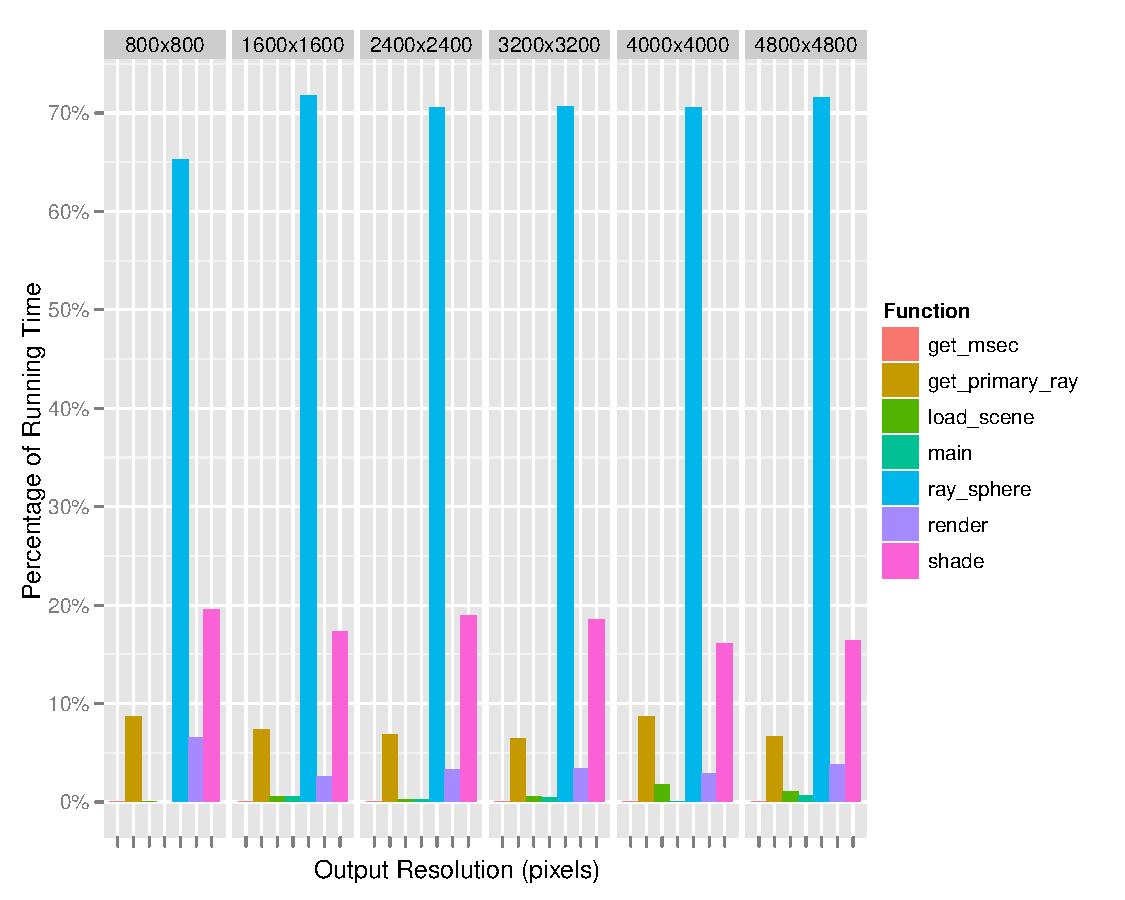
\includegraphics{cudatrace-002}
    \end{center}
\end{figure}


Using the knowledge of Tesla M2050 specifications, we can divide ray generation between the 14 SMs (448 CUDA cores $\times$ 1 SM/32 CUDA cores). On top of the parallelism of a single thread per SM, we can run multiple threads per SM. This would allow us to theoretically run 21,504 maximum threads (14 SM $\times$ 1536 threads/SM), and trace the same amount of rays, in parallel. We later determine the optimum block size, or threads per block, to take advantage of the maximum amount of threads which can run in parallel.

In addition to determining how many threads per block will be tracing rays, we will also have to optimize locality of the pixel data each thread needs. If we do not consider locality, each time a block runs out of stored pixel data to generate a ray, it has to fetch more data from the host. Because it takes more time to fetch data from outside of the kernel than inside, the accumulated transferring of data between the host and kernel will consume significant overhead and possibly trump the gains of computing in parallel. For this reason, we must distribute all of the pixel data necessary for each block to trace its maximum amount of rays before computations begin.

We have implemented \textsc{cudatrace} using NVIDIA's CUDA Developer Toolkit. This toolkit includes several useful tools for programming in CUDA as well as debugging code written using the CUDA API. The \texttt{nvcc} utility compiles CUDA/C or CUDA/C++ code in a format familiar to anyone who has used \texttt{gcc}. Similarly, \texttt{cuda-gdb} is a port of another familiar UNIX tool, the GNU Debugger, and is capable of debugging both native host code as well as CUDA code. The \texttt{cuda-memcheck} tool provides an interface for reporting runtime execution and memory access errors. Finally, NVIDIA's CUDA Profiler outputs the performance details of each individual CUDA API function call made.


\section{Initial Modification}
A significant portion of \textsc{cudatrace}'s primary modifications consisted of CUDA API function call additions to allocate and transfer memory between the host and device prior to and following the rendering of a scene by means of ray-tracing. A brief description follows of CUDA's conventions for obtaining parallelism and the purpose of CUDA API functions. Before any parallel computation can begin, the kernel must have access to all of the data it will utilize. The kernel does not have access to any malloc-allocated memory in the host, so a specific CUDA API function call must be made to allocate kernel-specific memory, called \texttt{cudaMalloc}. Similarly, cudaFree is used to free any memory allocated with \texttt{cudaMalloc}. This memory still cannot be seen by the kernel until it is passed as an argument into the kernel call. In order to transfer data between host-allocated memory and the kernel-allocated memory, the \texttt{cudaMemcpy} function is used. The first kernel function called must have a \texttt{\_\_global\_\_} prefix added to its definition, and it always takes as an argument the number of threads per block and the number of blocks to be used. Additionally, any functions called within the kernel must have a \texttt{\_\_device\_\_} prefix.    

With these conventions for parallelism in mind, figures \ref{code:c-ray_basic} and \ref{code:cudatrace_basic} compare how C-Ray and \textsc{cudatrace} call the function to initialize ray-tracing and transfer output data into an image file.

\begin{figure}[H]
    \caption{\textsc{cudatrace} version} \label{code:cudatrace_basic}
\begin{lstlisting}
...
allocate host memory for frame buffer array

call render1 function, which allocates and transfers kernel memory for ray-tracing
 
print image resolution to image file

for each color output/pixel data contained in the frame buffer
write the RGB values to the image file
}
...

render1 function
{
     calculate number of threads per block and number of blocks
  
     allocate kernel memory for kernel version of frame buffer, flattened object list, number of objects, camera, lights list    
    
    transfer host memory to kernel memory for flattened object list, number of objects, camera, lights list

     call the kernel, which begins the ray-tracing (provide arguments including number of blocks, threads per block, and all of the kernel memory previously allocated)

     copy kernel memory output data from kernel frame buffer to host frame buffer

     free all allocated kernel memory
}  

\end{lstlisting}
\end{figure}

\begin{figure}[H]
    \caption{C-Ray version} \label{code:c-ray_basic}
\begin{lstlisting}
...
allocate host memory for frame buffer array

// begin ray-tracing
call render function 


print image resolution to image file

for each color output/pixel data contained in the frame buffer
write the RGB values to the image file
...
\end{lstlisting}
\end{figure}

As seen in the pseudocode, the primary difference between C-Ray and \textsc{cudatrace} is that separate pointers or arrays must be created for each variable which will be read in the kernel. Consequently, we created a separate function, render1, to allocate and transfer memory for these pointers and arrays. Both \textsc{cudatrace} and C-Ray are similar in that they transfer the color output contained in the host frame buffer to the image file following the ray-tracing. 

Also present in the \textsc{cudatrace} pseudocode is a calculation of the number of threads and the number of blocks. \textsc{cudatrace} divides each image up into two-dimensional blocks of 256 (16 by 16) threads, a number we initially chose to ensure relatively broad cross-platform compatibility when dealing with GPUs that have varying maximum thread per block limits. Each thread handles the tracing and rendering of one single pixel. These blocks in turn make up a two-dimensional grid of dimensions (image width divided by the number of threads) by (image height divided by the number of threads). Thus, the full grid encompasses the full resolution of the image by way of maximized parallelism. In the final implementation of \textsc{cudatrace}, we assess the benefits of more or fewer threads per block.

This led to at least one complexity in our render functions, as we now needed to store all of these pixels, already logically oriented in a grid as they should be, in a one-dimensional array. This proved to be a relatively simple task, given CUDA's support for thread, block, and grid indices. Once we calculated the $x$ and $y$ coordinates of the pixel currently being operated on, storing it was simply a matter of using a flattened index of the form “x times grid width + y”. The final remaining snag was dealing with those image resolutions that were not an even multiple of 16 (the number of threads per block in each dimension). In those cases, we simply add one more partially filled block to the total number of blocks in that dimension. As a result, in our rendering functions we have to check to ensure that our $x$ and $y$ coordinates are less than the $x$ and $y$ dimensions of the image we are rendering to make sure we do not go out of bounds or overflow. 

Aside from the modifications made in apparent in \textsc{cudatrace}'s pseudocode, we were forced to further restructure certain C-Ray functions to make up for limitations of CUDA architecture. For example, C-Ray creates a linked list of objects when it loads data from the scene file. C-Ray understandably uses a linked list to contain objects because it cannot determine how many elements will be in a scene and thus how much memory to allocate for a flat array prior to reading the scene file. However, as demonstrated in the pseudocode, each host memory allocation containing data which will be used by the kernel must have a corresponding kernel memory allocation. It would be impractical to suffer the overhead of a number of \texttt{cudaMalloc} calls equivalent to the number of objects in a scene, so we implemented a function which would create a flattened array of the host's linked list of objects. This flattened array memory is then copied to its corresponding kernel array in the aforementioned pseudocode. Figure \ref{code:flatten_obj_list} illustrates the function \texttt{flatten\_obj\_list}, which flattens a linked list of objects.

\begin{figure}
    \caption{\texttt{flatten\_obj\_list} implementation} \label{code:flatten_obj_list}
\begin{lstlisting}
flatten_obj_list function
{
   
    for each number of objects in the linked list 
   {
        add the linked list object to the flattened array
        define flattened array element to be not null
    }
    define next flattened array element to be null 
}
\end{lstlisting}
\end{figure}

This pseudocode shows that each sphere has a \texttt{not\_null} variable, which is set to true only if a given element of the flattened array contains an object. After each object in the scene has filled the flattened array, the final element of the array does not contain an object and thus sets the \texttt{not\_null} variable to false. This construction was necessary to account for C-Ray's loops which would continue to run until the linked list of objects pointed to an invalid object.

Another \textsc{cudatrace} modification included the removal of all C-Ray recursive function calls. This aspect of \textsc{cudatrace} was actually not necessary to successfully compile on the Tesla M2050 GPU, but we began the creation of \textsc{cudatrace} with the prospect of compiling on NVIDIA GPUs with a 1.3 compute capability. GPUs with a 1.3 compute capability restrict any form of recursive function calling, but GPUs with a 2.0 compute capability are free of this restriction. In C-Ray, indirect recursion occurs during the creation of reflection rays, in which the trace function calls the shade function if the ray traces to an object, which then calls the trace function if a reflection ray should be traced. If the current ray being traced hits an object, the reflection depth limits the amount of times reflection rays can be traced. In \textsc{cudatrace}, we prevented reflection rays from being traced until the original trace function had returned. Figure \ref{code:recursion_workaround} demonstrates our recursion workaround.

\begin{figure}
    \caption{Avoiding recursion in \textsc{cudatrace}} \label{code:recursion_workaround}
\begin{lstlisting}
...
 for each sample {      
            call trace function to determine output color(pass in as arguments reflection boolean and reflection ray data container)

            while reflection boolean is true(or while reflection rays should be traced) {
                call trace function to determine reflection color(pass in reflection ray container data as argument)
                sum up the reflection color and color values
            }
}
...

trace function {
    ...  
    if reflection depth is greater than or equal to the maximum reflection depth {
        all RGB colors are set to black
        reflection boolean is set to false(no more reflection rays should be traced)
        return color value
    }
   ...
   if nearest object is a valid object {
        call shade function to determine color(pass in as arguments reflection boolean and reflection ray data container)
   } 
   else {
        all RGB colors are set to black
        reflection boolean is set to false
   }
   ...
}

shade function {
   ...
   if object should have a reflection ray {
     reflection boolean is set to true(another reflection ray should be traced)
     data is stored in reflection ray data container
     depth in incremented
   }   
   else {
     reflection boolean is set to false
   }
   ...
}  
\end{lstlisting}
\end{figure}

As seen from the pseudocode, calling the trace function returns a color. If reflection rays must be traced, the returned color of each trace function is summed to obtain the final color. The function which calls trace passes \texttt{trace\_reflection\_ray} and \texttt{reflection\_ray\_data} pointers as arguments into trace. \texttt{trace\_reflection\_ray} is dereferenced and set to true in the shade function if another reflection ray must be traced. If a reflection ray must be traced, all of the necessary ray data which is passed into the following trace call is stored in the dereferenced \texttt{reflection\_ray\_data} pointer. When the call to trace returns and the output color is summed, a test is made to see if the dereferenced \texttt{trace\_reflection\_ray} is set to true. If so, the dereferenced \texttt{reflection\_ray\_data} ray is used as an argument to the following trace function.

By the time we had finalized initial modifications and had successfully compiled \textsc{cudatrace}, we were able to tap the source of parallelism we sought after in our model---that is, parallelism by means of tracing rays simultaneously. However, the limitations of CUDA, such as kernel call specifications, memory restrictions, and the inability to easily utilize linked lists; negated our ability to implement minor or modest changes in the initial version of \textsc{cudatrace}. We were forced to direct much of the programming effort into restructuring a portion of the code to match the CUDA programming paradigm.

To test the improvement between C-Ray and the initial \textsc{cudatrace} implementation, we ran a test suite that rendered images of varying resolutions with each version. The attached data set and graphs illustrate the results of our testing. In sum, for lower resolutions (roughly less than 2400 by 2400 pixels), we found that C-Ray was more efficient (by three orders of magnitude). For each of the resolutions tested below this limit, \textsc{cudatrace} took roughly 3 seconds to render. At the time, we hypothesized that this was due to the overhead involved with copying the scene data to and from the GPU. After running the CUDA profiler and performing further overhead experiments, we later discovered the true bottleneck source, which is explained in the following section. 


Above that 5.5 megapixel cutoff, however, the data changes drastically, and \textsc{cudatrace} far outpaces C-Ray. At 576 megapixels, the maximum resolution we were able to test out without running into memory allocation issues due to hardware limitations, \textsc{cudatrace} was able to render the image in around 90 seconds, a stark comparison to C-Ray, which took over seven minutes to complete. 

%INSERT INITIAL GRAPHS

Due to \textsc{cudatrace}'s impressive performance at high dimensions and the heavy code restructuring necessary to achieve this gain, we believed our initial version of \textsc{cudatrace} tapped much of the possible parallel performance increase available with C-Ray's program structure. Thus, it seemed unlikely after creating \textsc{cudatrace} that we would be able to obtain another performance increase of a similar magnitude without possibly modifiying the ray-tracing algorithm and the data types used. For the final version of \textsc{cudatrace}, instead of aiming for a drastic modification which would further decrease the time taken to render large scenes, we chose to determine what causing the bottleneck which prevented \textsc{cudatrace} from being more efficient than C-Ray at lower dimensions.

\section{Final Modification}
As we began the final phase of \textsc{cudatrace} modifications, we sought to improve upon what caused the initial version to run slower than C-Ray at dimensions under $2400 \times 2400$ pixels.  We were aware of three areas in which we could provide improvement. First, we knew that each CUDA API call had a certain overhead associated with it. Further research allowed us to determine that the total program API call overhead was primarily affected by the amount of memory being allocated or transferred in each CUDA API call. We had many unnecessary calls present in our initial modification which were remnants of previous implementations, and we accordingly planned to remove them. Next, we were able to determine using the CUDA profiler that most of the overhead was a result of the \texttt{cudaMemcpy} function which transfers the device output data to the host. In that manner, we sought to either lessen the time of this transfer or determine an alternative method to port the output data into an image file. Finally, we did not have time during the initial modification to record variations in performance in respect to thread and block amounts. We thus attempted to determine what these optimal amounts would be.

Of our 24 initial CUDA API functions, we were able to remove 10 of them. Many of the deleted calls transferred unnecessary data from the device to the host following the call to the kernel. However, a significant portion of the removed calls consisted of cudaFree functions. Our removal of these cudaFree calls was not significantly dangerous, considering we would not be allocating any further device memory afterward. However, the removal of these calls did not produce any notable  improvements. We also did not take into account that when the CUDA driver context is deleted at the end of every program runtime, all allocated device memory is automatically freed. Thus, it is likely that the removal of the cudaFree calls did not delete any overhead time from the entire program runtime. 

When looking to reduce the overhead of the memory transfer from the device to the host, we knew that we would not be able to decrease the amount of data being transferred without altering output quality. We were consequently restricted to either finding an element of the architecture which would allow for improved transfer speeds or avoiding the transfer of memory altogether. In terms of the latter, we could only evade a memory transfer if each device sent its output directly to the image file. However, CUDA restricts us from writing to files while in the kernel. Even if this was possible, the overhead of writing to disk from the GPU, which would be assumedly longer compared to a write from the CPU, would negate speed gains already obtained from tracing rays in parallel. 

In terms of accelerating transfer time using aspects of the architecture, we discovered a function called \texttt{cudaMallocHost} which perfectly fit our needs. The \texttt{cudaMallocHost} function allocates pinned memory in the host, which means that any memory allocated with this call cannot be overwritten unless the programmer creates code to explicitly do this. It also allows for allocated host memory to be tracked and aligned by the CUDA context, creating greater throughput during transfers of memory between the host and device. However, there is one drawback to \texttt{cudaMallocHost}: it is a magnitude of three to five times slower than malloc. 

At this point, we also considered having each thread write its output to the host after it had finished tracing a ray. Putting aside the complications of determining the appropriate frame buffer index on the host, we found overhead tests of the \texttt{cudaMemcpy} function on 2.0 compute capability cards which demonstrate that it would take more time to transfer data accumulatively in small packets compared to transferring the total amount of data in one run.\footnote{\url{http://www.cs.virginia.edu/\%7Emwb7w/cuda\_support/memory\_transfer\_overhead.html}}.

Comparing the program modifications between the initial and final versions of \textsc{cudatrace}, we believe more programming effort was exhausted in our primary restructuring of C-Ray to allow it to be compatible with CUDA's restrictions. The initial version required us to remove recursive function calls, linked list usage, and modify each function called in the kernel with the appropriate device function headers. In the final version, however, many of the edits involved changing one or very few lines of code. For example, thread and block numbers could be changed by altering the numbers where we input the thread dimensions. The implementation of cudaHostMalloc required a substitution of only one call to malloc with the appropriate CUDA  call. 

\section{Performance Evaluation}

In evaluating \textsc{cudatrace}, we hoped to compare C-Ray with \texttt{cudatrace} for variable block sizes as well as resolutions. To make this possible, we first modified our existing application so that it would accept block dimensions as a command-line argument in addition to output resolution. The end result being that \textsc{cudatrace} can be called with syntax like
            
\begin{lstlisting}[language=bash]
    ./cudatrace -i scenefile -o scene.ppm -s 800x600 -t 16x16
\end{lstlisting}

and render an 800 by 600 pixel image using $16 \times 16 = 256$ threads per block.

With this addition, we were able to use a custom shell script, \texttt{cudatrace-tester.sh}, to test cudatrace. To ensure rigor and accurate results, we ran the test suite three times. To explore the performance speedup of \textsc{cudatrace} with respect to C-Ray at varying output image sizes, we tested both for the following resolutions (in pixels): $64 \times 64, 160\times160, 240\times240, 480\times480, 800\times800, 960\times960, 1120\times1120, 1280\times1280, 1440\times1440, 2400\times2400, 4800\times4800, 8000\times8000, 9600\times9600, 11200\times11200, 12800\times12800, 14400\times14400, and 16000\times16000$. In addition, we tested \textsc{cudatrace} at the following block sizes for each of those image resolutions: $1\times1, 2\times2, 4\times4, 8\times8, 12\times12, 16\times16, 20\times20, 22\times22$.

For three runs, this test suite takes roughly three hours, with much of the time spent rendering large images at small block sizes in \textsc{cudatrace} and in C-Ray. Under ideal circumstances, we would have tested both tracers at more image sizes to ensure good data resolution, but for our purposes this was sufficient.

The output of the test script is a comma-separated values (CSV) file with rows containing columns expressing the width and height of the output image, the $x$ and $y$ dimensions of the CUDA blocks, the render time, the real time, the application type (CUDA or sequential), and the run number. The distinction between render time and real time is important. The latter is simply the ``wall time'' for the program's execution: the time is noted at the initial command-line call and after the application returns; the difference between the two times is the real time taken. This includes I/O, CUDA context initialization overhead, and all other delays relevant to the execution of an application. The render time, on the other hand, attempts to prevent some of these factors from playing a role.  In the case of C-Ray, this time is only the time taken to trace all of the rays. Crucially in \texttt{cudatrace}, render time is simply the time taken to copy the stored scene information to the GPU, trace all necessary rays, and copy the result information back to the host.

\begin{figure}
    \caption{Render Time versus Real Time} \label{fig:render_vs_real}
    \begin{center}
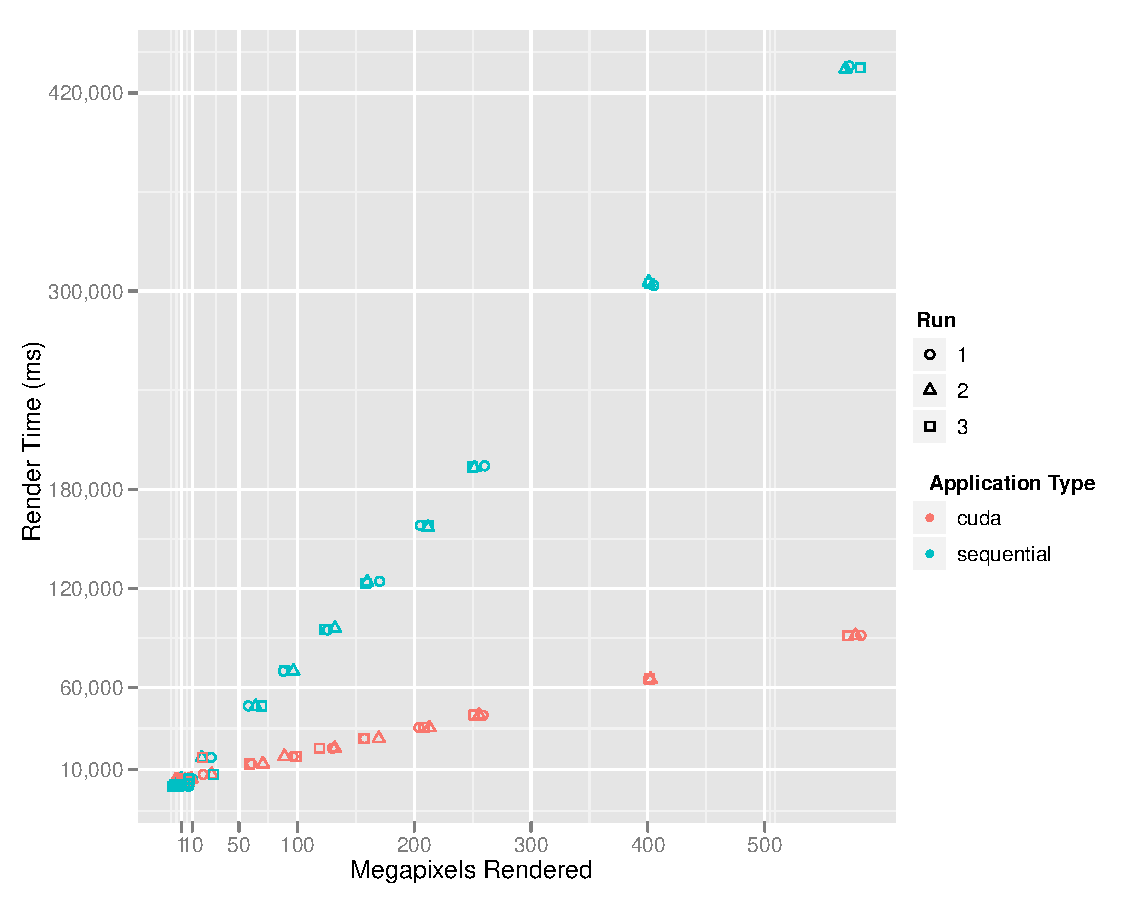
\includegraphics{cudatrace-003}
    \end{center}
\end{figure}


Crucially, the first call to the CUDA API occurs outside of this render time, eliminating from our performance analysis the unavoidable 3.5 second initialization time taken for the CUDA drivers to recognize the presence of a GPU and begin communicating with it. We discovered this quirk when trying to optimize \textsc{cudatrace} at low image resolutions. We found that there seemed to be an asymptotic lower limit to the real time that we were able to achieve around 3.5 seconds. To test if this latency was indeed the result of so-called context initialization, we wrote a small program to simply run \texttt{cudaFree(0)} once on the device and timed it using the same method as we had in our earlier evaluations. We found that this driver call, the only CUDA call in the test program, indeed took roughly 3.5 seconds to run on our test platform. Unfortunately, with the current structure of CUDA architecture, there is no way to initialize the CUDA driver and context before a program runs. The CUDA context normally initializes and is deleted with each CUDA program run. Having thus verified the source of our most significant bottleneck, we focused on optimizing render time and less of an emphasis on real time.

\begin{table}
    \caption{Context Initialization Time---Tesla M2050 GPU} \label{tab:warmup_time}
    \begin{center}
        \begin{tabular}{r | c}
            \toprule
            Run & Warmup Time \\
            \midrule
            1 & 3464 \\
            2 & 3426 \\
            3 & 3517 \\
            4 & 3422 \\
            5 & 3414 \\
            \bottomrule
        \end{tabular}
    \end{center}
\end{table}

We imported our test data into R and added some additional variables. We calculated both real speedup and render speedup as the time that C-Ray took divided by the time \texttt{cudatrace} took, for each iteration. We also trivially calculated the total pixels and total threads for each run. We used the ggplot package to provide some interesting visualizations.


\begin{figure}
    \caption{Real Speedup versus Megapixels} \label{fig:real_speedup}
    \begin{center}
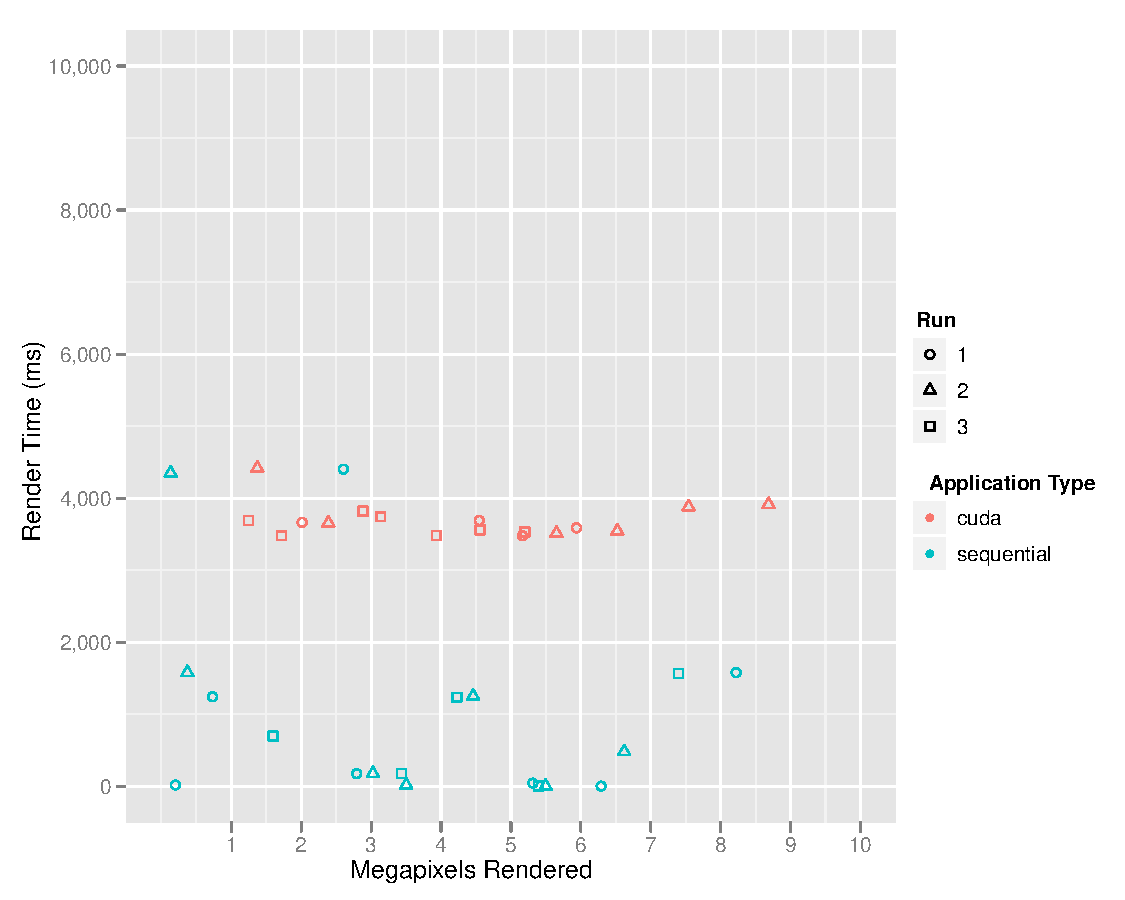
\includegraphics{cudatrace-004}
    \end{center}
\end{figure}

\begin{figure}
    \caption{Render Speedup versus Megapixels} \label{fig:render_speedup}
    \begin{center}
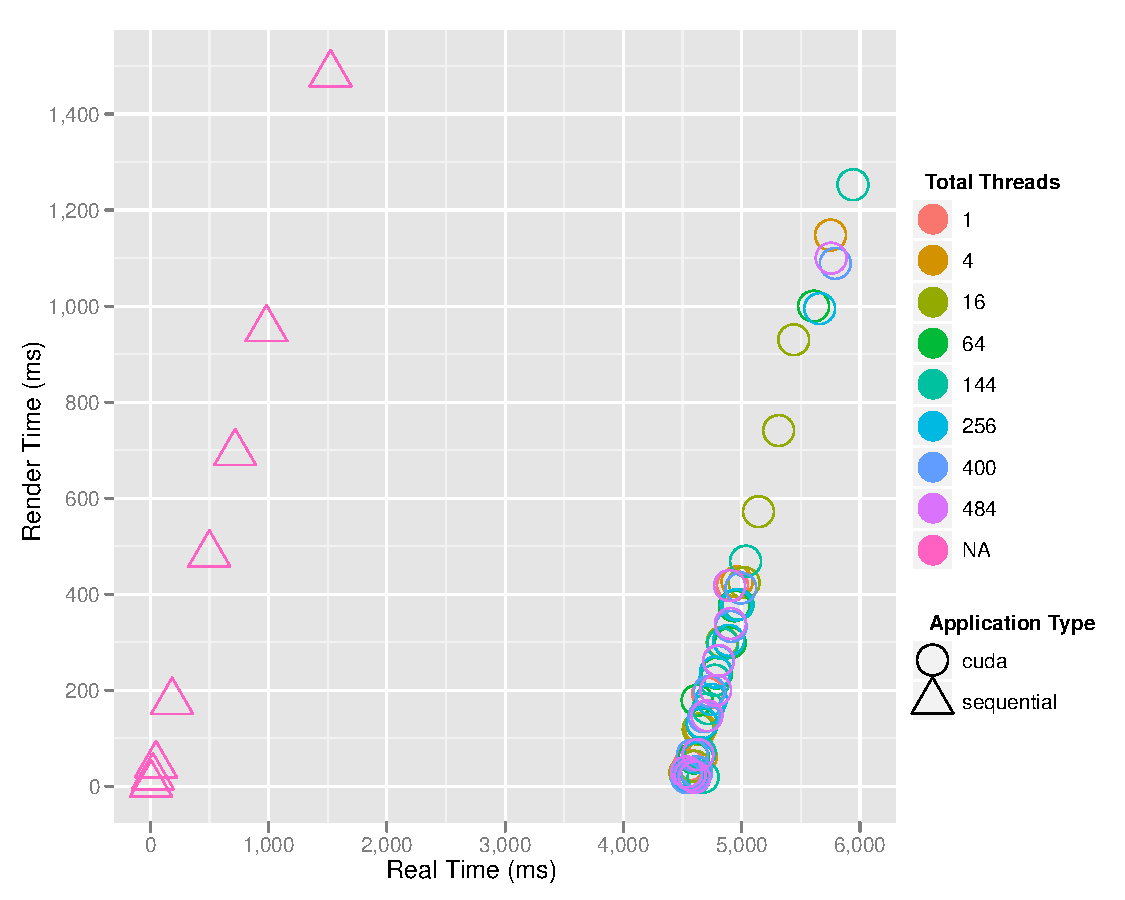
\includegraphics{cudatrace-005}
    \end{center}
\end{figure}

On the surface, it is very clear that our parallelized ray tracer performs better than C-Ray. In real time, we were able to realize a maximum speed up of -Inf for a $16000\times 16000$ pixel image. When measuring render time, we saw an even more impressive maximum of -Inf speedup for a $1280 \times 1280$ pixel image. This does not tell the whole story however. The number of threads per \textsc{cudatrace} execution played a significant role in determining the speedup.

\begin{center}
% latex table generated in R 2.14.0 by xtable 1.6-0 package
% Sat Dec  3 02:10:38 2011
\begin{table}[ht]
\begin{center}
\begin{tabular}{rrrrrr}
  \hline
 & Resolution & Real Speedup & Render Speedup & Minimum Threads & Maximum Threads \\ 
  \hline
1 & 64.00 & 0.00 & 0.22 & 16.00 & 400.00 \\ 
  2 & 160.00 & 0.00 & 0.86 & 64.00 & 256.00 \\ 
  3 & 240.00 & 0.01 & 1.67 & 64.00 & 64.00 \\ 
  4 & 480.00 & 0.04 & 3.00 & 64.00 & 144.00 \\ 
  5 & 800.00 & 0.11 & 3.74 & 64.00 & 64.00 \\ 
  6 & 960.00 & 0.16 & 3.91 & 64.00 & 64.00 \\ 
  7 & 1120.00 & 0.21 & 4.09 & 64.00 & 64.00 \\ 
  8 & 1280.00 & 0.31 & 4.96 & 64.00 & 64.00 \\ 
  9 & 1440.00 & 0.33 & 4.21 & 64.00 & 64.00 \\ 
  10 & 2400.00 & 0.80 & 4.51 & 256.00 & 256.00 \\ 
  11 & 4800.00 & 1.98 & 4.54 & 256.00 & 256.00 \\ 
  12 & 8000.00 & 2.90 & 4.58 & 256.00 & 256.00 \\ 
  13 & 9600.00 & 3.22 & 4.65 & 256.00 & 256.00 \\ 
  14 & 11200.00 & 3.39 & 4.67 & 256.00 & 256.00 \\ 
  15 & 12800.00 & 3.51 & 4.66 & 256.00 & 256.00 \\ 
  16 & 14400.00 & 3.58 & 4.65 & 256.00 & 256.00 \\ 
  17 & 16000.00 & 3.64 & 4.63 & 256.00 & 256.00 \\ 
   \hline
\end{tabular}
\caption{Maximum Speedup by Resolution}
\label{tab:max_speedup_each_res}
\end{center}
\end{table}\end{center}

\begin{figure}
    \caption{Inset---Render Speedup versus Megapixels} \label{fig:render_speedup_zoom}
    \begin{center}
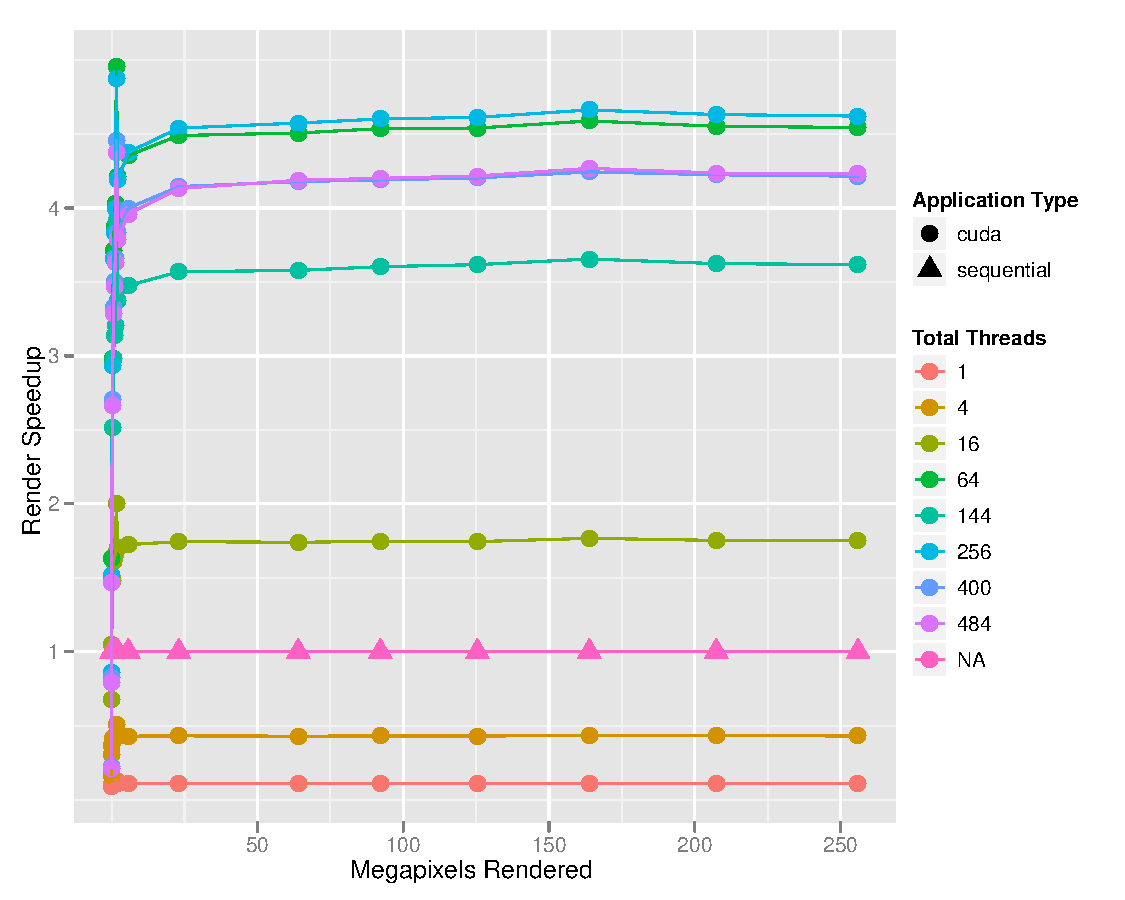
\includegraphics{cudatrace-007}
    \end{center}
\end{figure}

We did not see a real speedup for anything in our test suite below $4800 \times 4800$ pixel images, where we found a maximum real speedup of 1.977. Above that resolution however, we did see real speedups in all block sizes from 4x4 through $22 \times 22$. The $1 \times 1$ and $2 \times 2$ block sizes fell short of providing us with any improvement, as expected. For render time, we saw speedups in the same range of block sizes, but at a much lower starting resolution. At $240 \times 240$ pixels we saw render speedups ranging from approximately 1.05 for 4x4 threads to near 1.65 for $8 \times 8$ threads and just below that for 16x16 threads. We conclude that the significant difference in the ``break even'' point between real and render time is almost completely the result of the context initialization overhead inherit to CUDA and discussed previously. The less significant difference between the render speedup break even point of approximately $240 \times 240$ pixels can almost certainly be attributed to the overhead of allocating space on the CUDA device for the various components of the scene as well as copying the pixels frame buffer back from the device at the completion of all ray tracing calculations. As discussed earlier in this paper we believe we have reached a plateau in the potential optimizations of this element of the application. Because of this, we now address the render speedup in slightly more detail.

Despite the fact that there was some variation in the number of threads that gave the best performance at various resolutions, there was a clear pattern to the optimized block sizes. Overall, the most efficient number of threads was $16 \times 16 = 256$. This is directly tied to the hardware we did our testing on, the Tesla M2050 GPU. For \textsc{cudatrace} render time, reading and writing to memory are the highest latency operations executed, so the more threads we are able to run in parallel, the better we are able to disguise this latency. The M2050 have a CUDA compute capability of 2.0 and thus a maximum of 48 warps per multiprocessor (MP), eight thread blocks per MP, and 1536 threads per MP. Additionally, there is a physical limit of 32 threads per warp. Thus, for cases where overhead is not dominant, the optimal block size is that which maximizes the occupancy of each multiprocessor, or 1536 threads total.  In our case, this amounts to utilizing $1536/32 = 48$ warps per multiprocessor, the maximum. When we have $16 \times 16 = 256$ threads, we use $256 \times (6 \text{blocks}) = 1536$ active threads per multiprocessor, 100\% of the number of threads allowed on each multiprocessor. On the other hand, when we have $22 \times 22 = 484$ threads, we use $484 \times (3 \text{blocks}) = 1452$ threads per multiprocessor, only 94\% of the maximum number of threads. The maximum number of threads per block on CUDA 2.0 cards is 512. To comply with our use of two dimensional thread blocks, this would require an illegal block size of $22.63 \times 22.63$. Thus, 16x16 is the maximum block size that we can utilize with 100\% multiprocessor occupancy.

\begin{figure}
    \caption{Inset---Real Time versus Megapixels} \label{fig:real_time_zoom3}
    \begin{center}
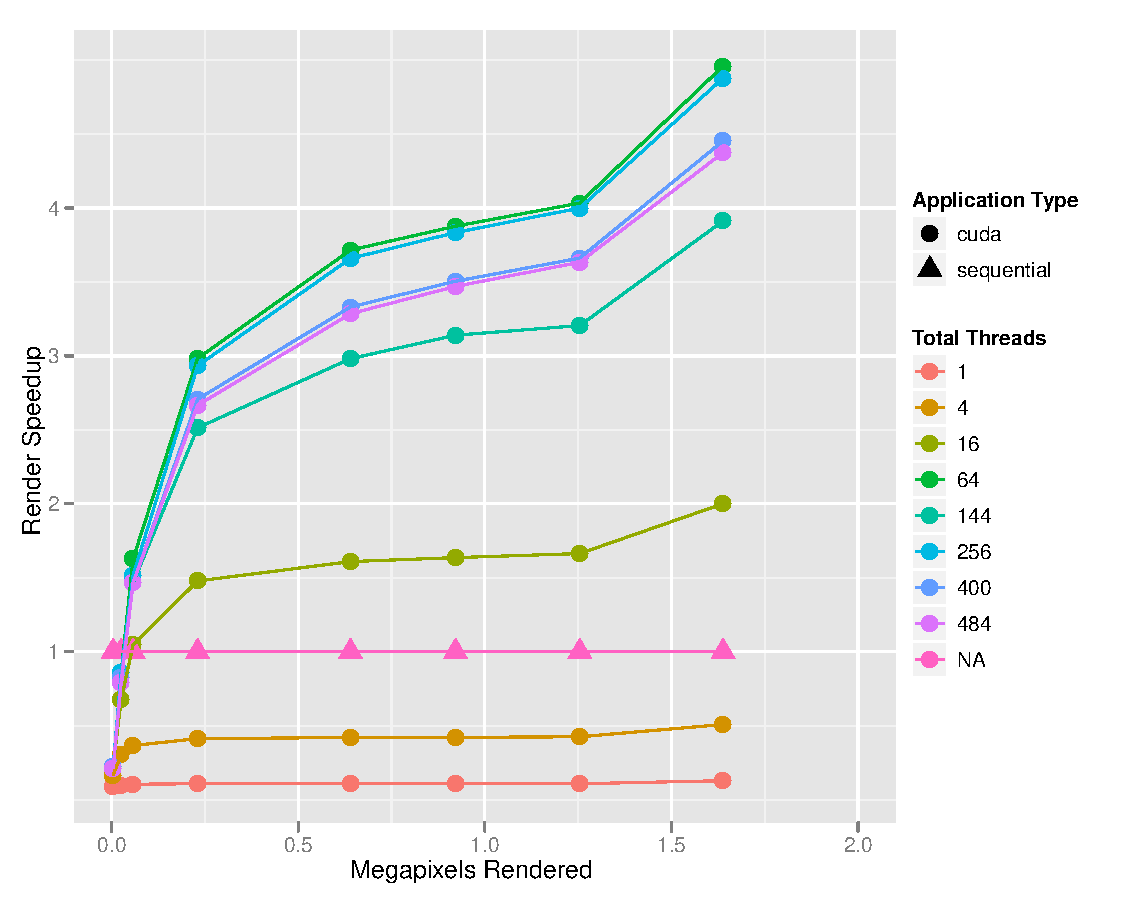
\includegraphics{cudatrace-008}
    \end{center}
\end{figure}

For image resolutions below $2400 \times 2400$, we found that block sizes of 8x8 were actually slightly more efficient than those of 16x16 despite the fact that the former only reaches 33\% occupancy. We attribute this to the added overhead required to create four times as many threads for such a relatively small resolution. Note that the render speedup difference between 8x8 and 16x16 in this range is on the order of magnitude of 0.1. Above $2400 \times 2400$, $16 \times 16$ threads reigns supreme, although a block size of $8 \times 8$ only lags behind by approximately 0.1 with regard to render speedup.

\begin{figure}
    \caption{Inset---Render Time versus Megapixels} \label{fig:render_no_jitter_time_zoom3}
    \begin{center}
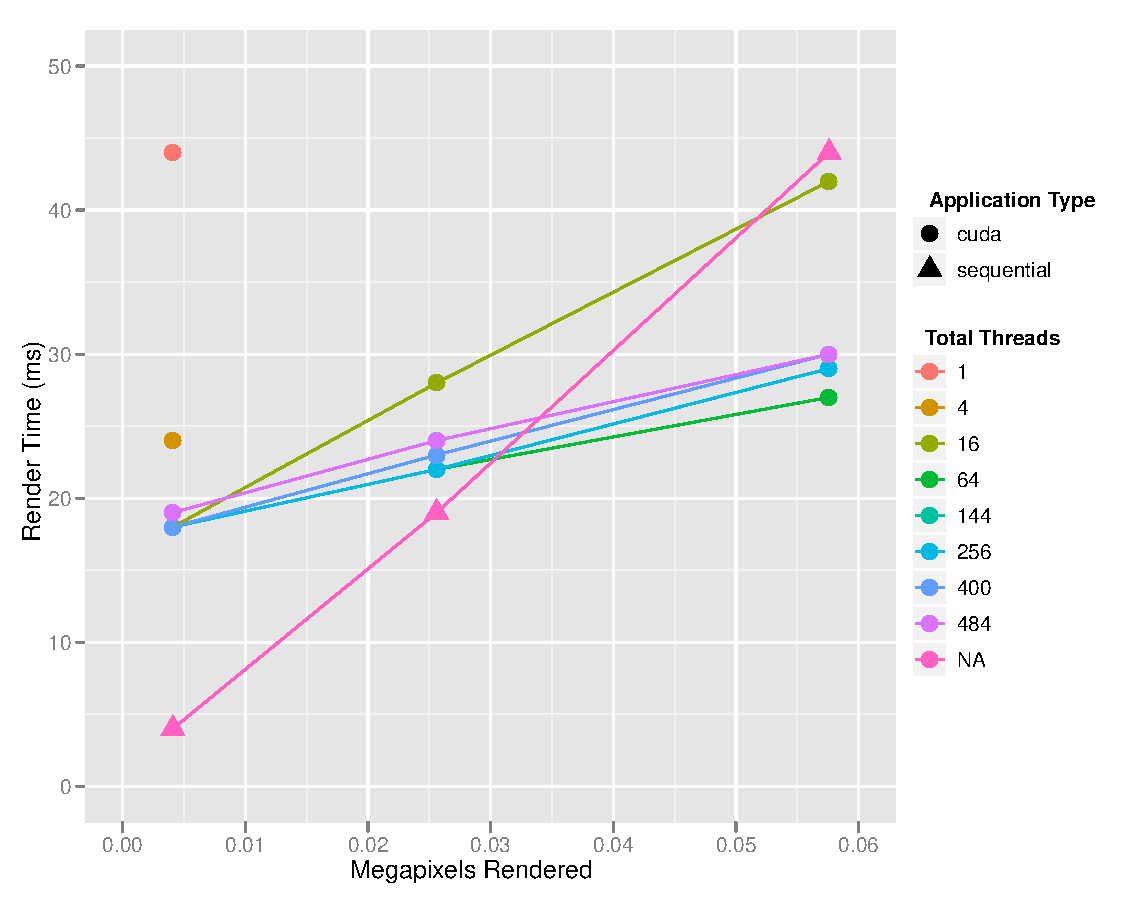
\includegraphics{cudatrace-009}
    \end{center}
\end{figure}

Acknowledging that our greatest barrier toward having \textsc{cudatrace} outpace C-Ray at any given frame dimension was the overhead of context creation, we considered the possibility of sequentially tracing rays for all given dimensions under $2400 \times 2400$ pixels. This could be implemented by importing all of C-Ray's functions which are involved in ray rendering. The function could then test if the given dimensions are under $2400 \times 2400$ pixels. If under this amount, the host frame buffer would have memory allocated using malloc and each ray would be traced sequentially using C-Ray's original functions. If above this amount, the host frame buffer would have memory allocated using \texttt{cudaMallocHost}, and a context would be created. All of the required scene information would be have memory allocated in the kernel, and the kernel call would be made, allowing each ray to be traced in parallel. Drawbacks of this implementation include increased program size, increased compile time, and a lack of parallel exploitation as NVIDIA creates cards with decreased CUDA API call and context overhead. 

\section{Limitations of CUDA and Project Conflicts}

As we searched for methods to improve \textsc{cudatrace}'s performance, we came across a variety of brick walls which were mostly the fault of the GPU hardware. For example, CUDA driver and context initialization overhead time constituted one of our greatest bottlenecks when rendering scenes under $2400 \times 2400$ pixels. 

Additionally, both \textsc{cudatrace} and C-Ray fail at very high resolutions (over approximately 600 megapixels) because we attempt to store all of the frame buffer pixels in memory at the same time. It is possible to overcome this by writing to the file in blocks as the rendering occurs, rather than all at once after all rays are traced. However, the accumulated overhead of multiple \texttt{cudaMemcpy} calls would swiftly overtake the overhead of a single \texttt{cudaMemcpy} call which transferred the entirety of the output data to the host frame buffer. Assuming we ignored this drawback, our next hardware-related ceiling is the GPU's limitation on number of thread blocks allowed in the grid. For modern hardware, this will not quickly become an issue, as CUDA  supports 65,535 times 65,535 = 4,294,836,225 blocks. With our conservative implementation of 256 threads per block, each handling one pixel, we are left with a rough theoretical maximum of 1.09 trillion pixels. 

The final hardware limitation we noted affects the processing of double-precision variables. The rendering of each ray involves computation on a significant amount of 3-tuple structures. Each element of a 3-tuple is a double.  Using a CUDA 2.0 compute capability GPU, only one double-precision operation can be performed per cycle per core. Thus, our double-precision variables limit the amount of parallelism we are able to exploit.

Each of the mentioned limitations may currently represent insurmountable bottlenecks, but they will more than likely become less prominent as NVIDIA continues to release GPUs with hardware improvements. However, we are not guaranteed that future GPU architectures will be backwards compatible, so we may pay the price of restructuring \textsc{cudatrace} to take advantage of future hardware improvements.

\section{Choices and Tradeoffs}

The ``end'' of Moore's Law has largely dictated that computer architects develop new ways of increasing application speed without vastly multiplying the number of transistors on the CPU. For applications that are able to utilize it, parallel programming offers irrefutable benefits to the end-user: speed, energy efficiency, and throughput. Many of the tradeoffs come in the form of new complications for developers however. Programming in parallel is an entirely different paradigm from sequential programming, and implementations must utilize different algorithms, different management of data,  and more attention to hardware specifications. Whereas sequential programs rarely have specific dependencies on the hardware level behind the general architecture (x86 versus MIPS for example), many of the latest and greatest software interfaces utilized in parallel programming bring with them entirely new hardware devices as well: GPGPU programming requires a graphics card, OpenMP utilizes multi-core systems, MPI employs an entire cluster, etc.       

While new hardware with tightly integrated software interfaces seems to be a necessity for any notable improvement in speed and efficiency, the wide array of varying contenders for ``the future'' of programming makes it difficult for developers to harness any of them in creating applications for mainstream customers. The vast majority of personal computers have normalized to a few different architectures allowing programmers to focus on optimizing for them specifically with the assistance of compilers. Developing parallel implementations that utilize GPUs, multi-core systems, and clusters is far too much to expect of programmers in most cases, especially because there is no guarantee that the hardware that is targeted will still be relevant even a year after release. Software developers thus have to choose between improving performance and alienating users, or stagnating and guaranteeing support for almost everyone. The general ubiquity of multi-core systems offers some hope in this regard, but still no guarantees. For parallel programming to truly become worth investing in  the necessary time for developers, there needs to be greater assurance that their investment will be beneficial in the long-term and for a majority of their target audience. Until parallel architectures become more common, this will restrain their utilization to developers working in high performance computing fields. 

\section{Looking Forward}
The experience of developing \textsc{cudatrace} has brought to our attention several of the potential benefits as well as some of the difficulties involved with GPGPU programming. Our difficulties in finding a consistent and reliable testing platform for our relatively simple application exhibit one of the most prominent issues opposing CUDA's attempt to become relevant for more mainstream computing. The initial public version of CUDA was released in early 2007. In the four short years since version 1.0, NVIDIA has released five new iterations of CUDA with varying degrees of backwards-compatibility. Further, despite the fact that in some cases there may not be physical limitations that require it, NVIDIA has chosen to restrict hardware devices to specific compute capabilities, thus shortening the period of compatibility even more. This factor alone presents a serious problem as to the long term viability of CUDA as a platform in areas other than scientific research or academia. Unless NVIDIA develops a more stable hardware-software interface, software developers are likely to pass it up for more reliable architectures guaranteed to be usable on a variety of devices for a significant length of time.

Beyond that (significant) issue, the integration of CUDA and C/C++ provides a convenient entry point for developers looking to parallelize their code. Our experiment has shown that properly optimized code that takes full advantage of the number of cores available on a given GPU can offer truly dramatic improvements over sequential counterparts.

As an demonstration of the potential use for CUDA in graphics-heavy application like video games and computer generated imagery, consider this: for the equivalent of full high definition imagery and without the context initialization time overhead, \textsc{cudatrace} is able to generate nearly three frames per second. For the much smaller image size of 240x240 pixels, \textsc{cudatrace} is able to render images approximately frequently enough to appear like real-time output to the human eye ($\approx 25$ frames per second). While this resolution may seem comically small, the actual ray-tracing computations of our starting point (C-Ray) are far from optimized. Further, had we chosen to sacrifice accuracy and utilize single precision floats instead of double precision, a change that might be acceptable in a real-time tracer, we would have seen significant gains as existing CUDA hardware is optimized for the former. Hardware advances as well as more well-integrated GPU systems will address the context initialization issues and cut down on the other elements of overhead inherent to CUDA at this point, further aiding performance.

The comparatively low cost and ease of obtaining a GPU (which may be included with your computer in the first place) as opposed to creating a cluster (for MPI) or obtaining a many-core CPU provides a notable benefit for GPGPU programming. CUDA provides a compelling hardware-software interface for developers, but the fast-paced rate at which NVIDIA has chosen to release major changes to it has rendered it impractical for many outside of research and high performance computing communities. Because of this factor, we predict that GPGPU programming and CUDA specifically will struggle to gain mainstream acceptance in the near future. The ease of which massively parallel applications can be composed provides a compelling enough argument for the persistence of GPGPU programming, however, and we speculate that as the field stabilizes and cross-platform compatibility becomes more common, this architecture will gain more widespread use.
\end{document}
